\documentclass{article}
\usepackage[utf8]{inputenc}
\usepackage{graphicx}
\graphicspath{ {c:/user/Acer/desktop/faks/matematično modeliranje/projekt} }
\usepackage{mathtools}
\usepackage{amssymb}
\usepackage{amsmath}
\usepackage{eurosym}

\begin{document}
\begin{titlepage}
   \begin{center}
       \vspace*{1cm}
 
       \textbf{\Huge{Bezierjeva krivulja in njen odmik}}
 
       \vspace{0.5cm}
        \Large{Poročilo projekta pri predmetu Matematično modeliranje}
 
       \vspace{1.5cm}
    \vfill
       \textbf{Maruša Oražem}
 
       
 \begin{figure}[!ht]
\centering
       
\includegraphics{fmf.png}
\end{figure}
 
       \textsc{\large{Univerza v Ljubljani}}
    
        \textsc{\large{Fakulteta za matematiko in fiziko}}
    
     \textsc{\large{Oddelek za matematiko}}
    \vfill\vfill
 
   \end{center}
\end{titlepage}






\tableofcontents











\newpage

\section{Predstavitev}
V nalogi so predstavljene Bezierjeve krivulje. Le te dobimo s pomočjo de Casteljauovega algoritma, ki je osnovni algoritev pri konstrukciji Bezierjevih krivulj. Poleg tega naloga vključuje tudi odmik Bezierjeve krivulje, to je krivulja, ki jo dobimo tako, da vsaki točki originalne krivulje priredimo novo točko v normalni smeri na oddaljenosti za neko konstanto d.


\section{de Casteljauov algoritem}
De Casteljavou algoritem je osnovni algoritem, s pomočjo katerega izračunamo vrednost točke na Bezierjevi krivuljio.
Razvil ga je Paul de Casteljau (rojen leta 1930 v Franciji), francoski fizik in matematik.

\subsection{Primer poteka algoritma}
Za lažjo razlago, si oglejmo primer. \\
Imamo podane kontrolne točke $P_0=(0,5),P_1=(1,-1),P_2=(3,0),P_3=(4,3),P_4=(6,10)$ in parametr $t=3/4$. \\
V prvem koraku definiramo $b_{j}^{0} := P_{j},j=0,1,2,3,4$. \\
Potem računamo $b_{j}^k(t) :=(1-t)b_{j}^{k-1}(t) + tb_{j+1}^{k-1}(t), k = 1,...,4, j = 0,1,...4-k$.
Rezultat $b_{0}^4(t)$ je točka na Bezierjevi krivulji.\\
Slika spodaj prikazuje potek zgornjega postopka. \\
Črna barva predstavlja začetne točke (kontrolni poligon) oziroma prvi korak, rdeča barva končno Bezierjevo krivuljo, naslednji koraki si sledijo z modro barvo, oranžno in rumeno. Z zeleno zvezdico je označena končna izračunana točka.

 \begin{figure}[!ht]
\centering
       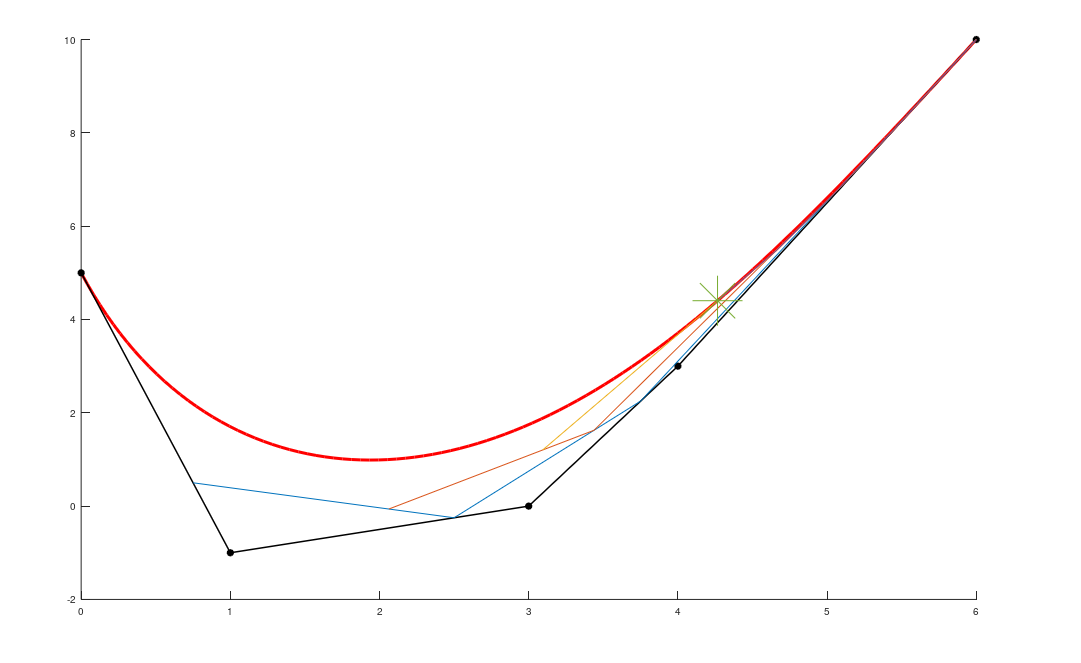
\includegraphics[width=120mm]{koncna.png}
\end{figure}




\subsection{Algoritem}
\textbf{Vhodni podatki:} $P_0,...,P_n\in R^n, t\in [0,1]$. \\
\textbf{Definiramo:} $b_j^0(t) = P_j$,\\
\textbf{Ponavljamo:}  $b_{j}^k(t) :=(1-t)b_{j}^{k-1}(t) + tb_{j+1}^{k-1}(t), k = 1,...,n, j = 0,1,...n-k$.\\
\textbf{Izhod:} $b_0^n(t)$ točka na krivulji.\\


Implementacija algoritma se nahaja v datoteki $deCasteljau.m$.
V datoteki smo vmesne točke shranjevali v matriko velikosti $(n+1)\times(n+1)$, kjer je $n$ število začetnih točk. Algoritem vrne končno točko na Bezierjevi krivulji.


\section{Bezierjeva krivulja}
Bezierjevo krivuljo dobimo s pomočjo de Casteljauvega algoritma in sicer tako, da izračunamo točke na krivulji za čimveč različnih parametrov. 
Datoteka $plotBezier.m$ nariše željeno krivuljo. Krivulja je definirana za parametr $t\in [0,1]$. Tako dani interval razdelimo na čimvečje število delcev in pokličemo de Casteljavou algoritem na vsakem posebej.


\section{Odmik krivulje}
Odmik je krivulja, ki jo dobimo tako, da vsaki točki originalne krivulje
priredimo točko, ki je na konstantni oddaljenosti d v normalni smeri.
Normalo na krivuljo dobimo tako, da najprej izračunamo tangento v dani točki, normala pa je premica, ki je pravokotna na tangentno.\\
\\
Izračun tangente v dani točki je vsebovan v datoteki $bezier\_der1.m$, izračun normale pa v $normala\_bez.m$. \\
Glede na to kako orientiramo krivuljo, imamo dve različi smeri normalnega vektorja. Normalni vektor je lahko obrnjen ali navznoter ali pa navzven. Pri izrisu "odmika" vidimo, da je slika veliko lepša, če normalo obrnemo navzven. Če jo obrnemo navznoter, pridejo zelo čudne stvari.
Spodaj je grafični prikaz Bezierjeve krivulje in njenega odmika, za enak primer začetnih točk in različne parametre.\\
Implementacija je vsebovana v datoteki $plot\_odmik$.
\newpage
 \begin{figure}[!ht]
\centering
       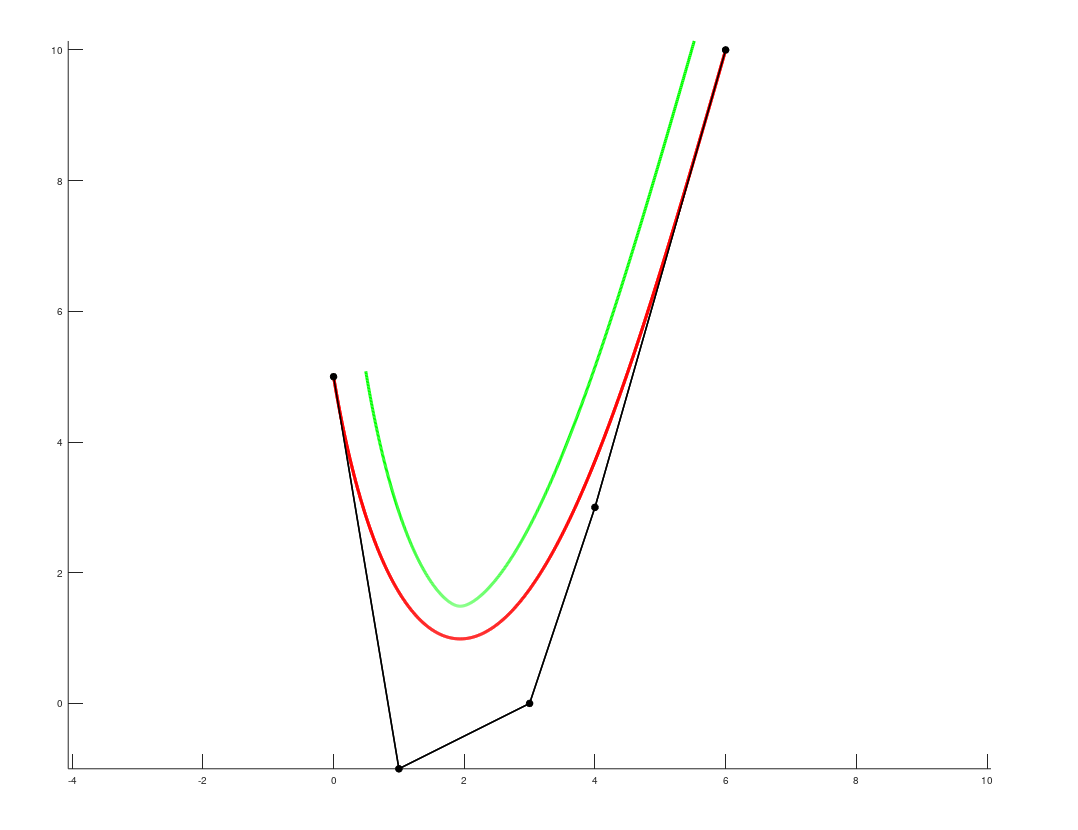
\includegraphics[width=70mm]{odmik1.png}
	\caption{Normala obrnjena navznoter, d = 0.5.}
\end{figure}

 \begin{figure}[!ht]
\centering
       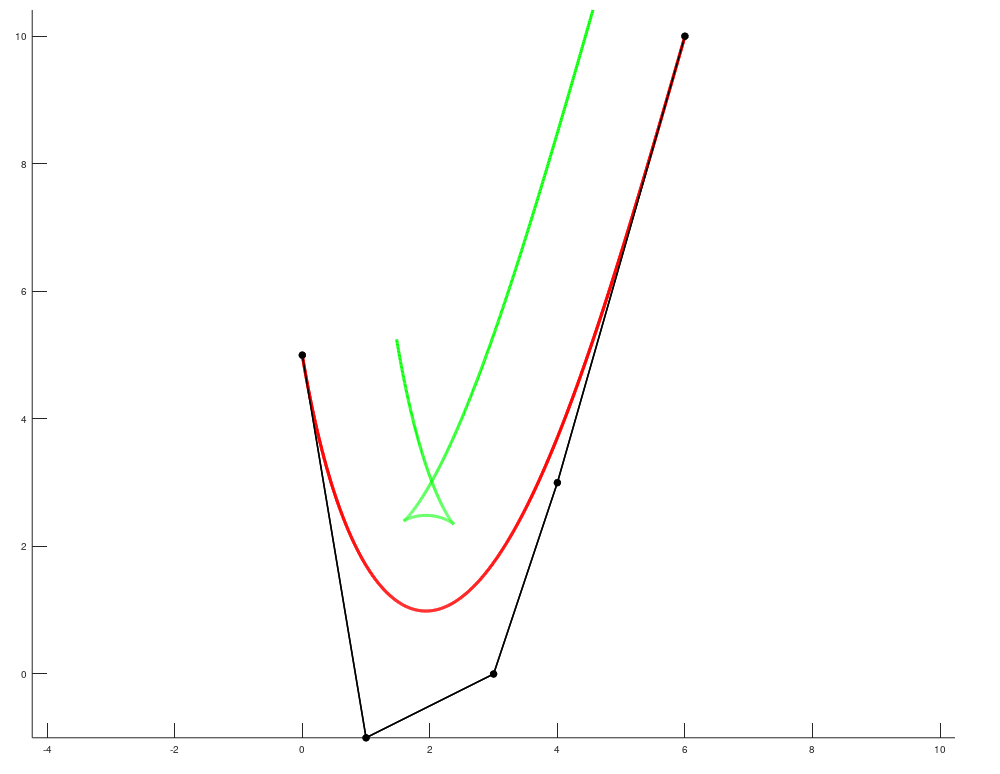
\includegraphics[width=70mm]{odmik2.png}
	\caption{Normala obrnjena navznoter, d = 1.5.}
\end{figure}

 \begin{figure}[!ht]
\centering
       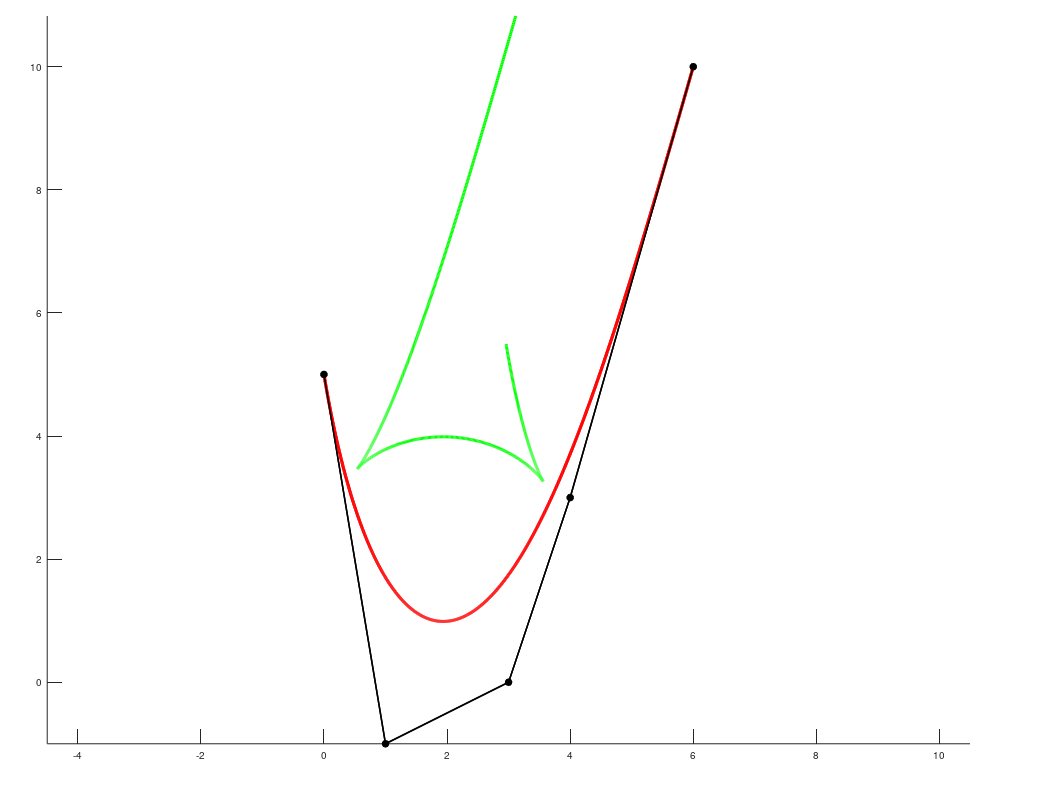
\includegraphics[width=70mm]{odmik3.png}
		\caption{Normala obrnjena navznoter, d = 3.}
\end{figure}

\newpage

 \begin{figure}[!ht]
\centering
       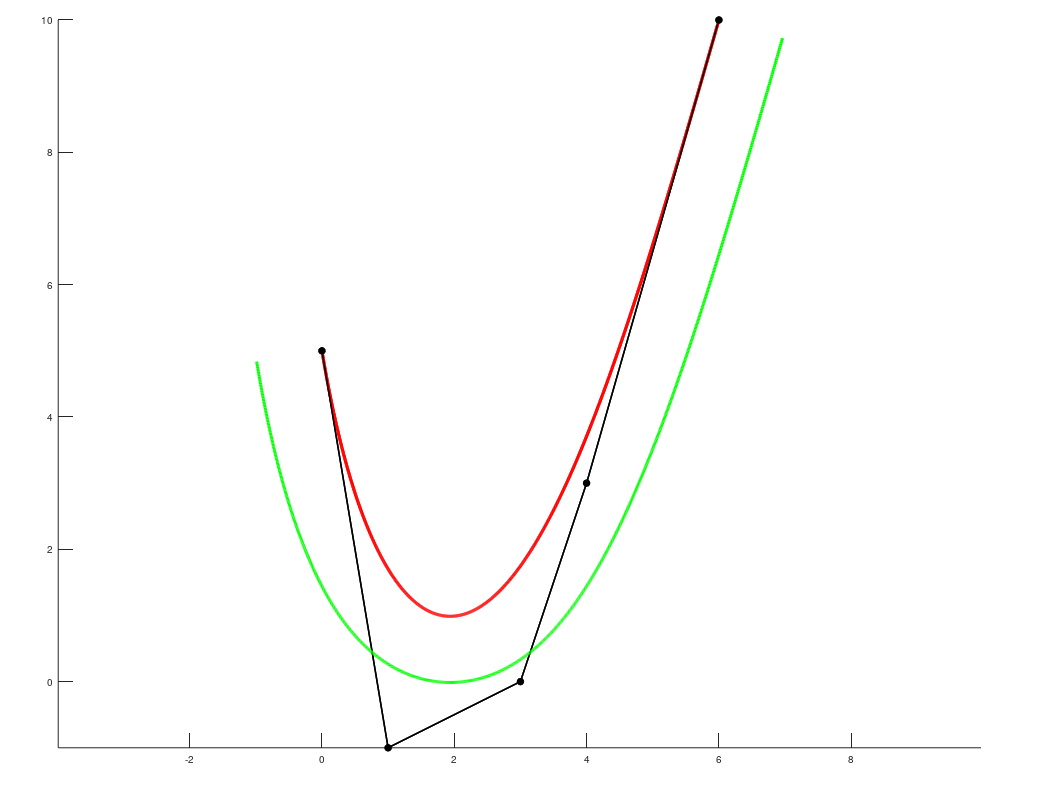
\includegraphics[width=70mm]{odmik4.png}
		\caption{Normala obrnjena navzven, d = 1.}
\end{figure}

 \begin{figure}[!ht]
\centering
       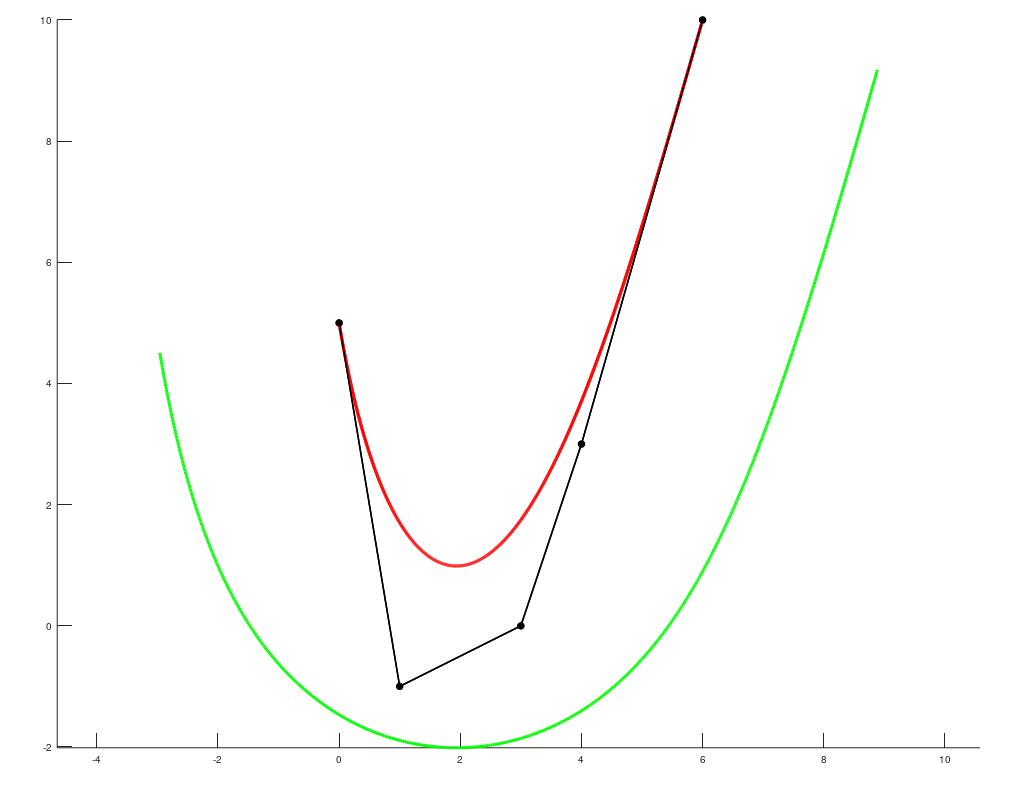
\includegraphics[width=70mm]{odmik5.png}
		\caption{Normala obrnjena navzven, d = 3.}
\end{figure}


\newpage
\begin{thebibliography}{9}

\bibitem{}
Žagar, E. Bezierove krivulje. 2009. [9.9.2019]. Dostopno na http://mars.dmfa.si/mars2009/folije/Predavanje-Zagar.pdf.


\end{thebibliography}





\end{document}
